\documentclass{article}
\usepackage[utf8]{inputenc}
\usepackage{amsmath}
\usepackage{amssymb}
\usepackage{graphicx}

\begin{document}

\section*{Solving a small linear system}
We have the following information: Daniel buys $3$ mangoes, $1$ kiwi, $7$ lychees and $2$ bananas. Peter buys
$2$ mangoes and $1$ pineapple. Julia needs $3$ pomegranates and $1$ mango for her fruit juice, whereas Ralf
needs $5$ kiwis and $1$ banana for his fruit salad. Marcus buys $1$ pineapple and $2$ bananas. Manfred buys $20$
lychees and $1$ kiwi. Daniel pays CHF $11.10$, Peter pays CHF $17.00$ (and so spends all his pocket money),
Julia pays CHF $6.10$, Ralf pays CHF $5.25$, Marcus pays CHF $12.50$ and Manfred pays CHF $7.00$.

\subsection*{2-1.a} We are tasked to refresh our knowledge on solving linear systems of equations (LSE) in Eigen. An LSE if of the form 

\begin{equation*}
    \mathbf{A}\mathbf{x} = \mathbf{b}
\end{equation*}
and its solution is given by
\begin{equation*}
    \mathbf{x}=\mathbf{A}^{-1}\mathbf{b}
\end{equation*}
however the usage of the function \verb|inverse| is discouraged as it is prone to numerical instability (or at least this is what we were told). We generally do the following 
\paragraph{$\mathbf{A}$ has no special structure:}
\begin{enumerate}
    \item We compute a decomposition of the matrix $\mathbf{A}$ (LU, QR, LLT LDLT, SVD).
    \item We then use the decomposition to perform backward and forward substitution by calling the existing \verb|solve()| method of the decomposition.
\end{enumerate}
\paragraph{LU-decomposition:} The LU decomposition can be used on \textbf{square} matrices $\mathbf{A}\in \mathbb{K}^{n,n}$ and decomposes the matrix $\mathbf{A}$ into an \textbf{upper triangular matrix} $\mathbf{U}\in \mathbb{K}^{n,n}$ and a \textbf{normalized} (all elements on the diagonal are equal to $1$) \textbf{lower triangular matrix}. 
\begin{figure}[!hbt]
    \centering
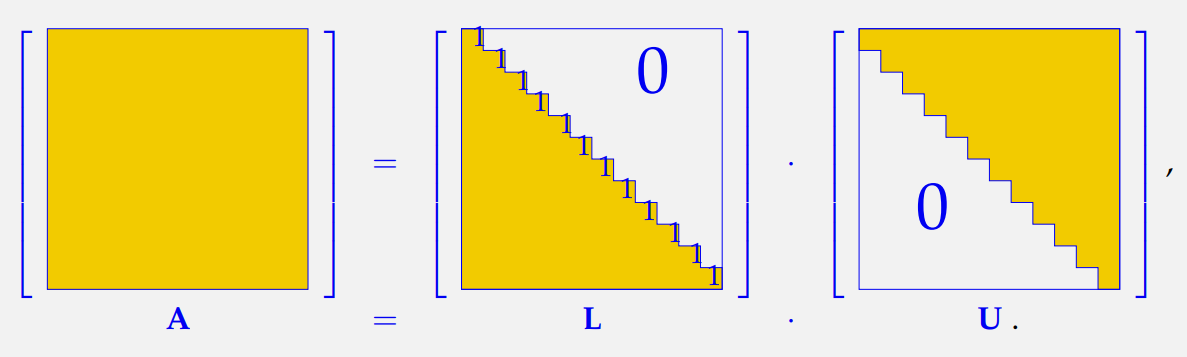
\includegraphics[width=1.0\linewidth]{LU-Decomposition.png}
\end{figure}

\noindent The Lu decomposition of a matrix $\mathbf{A} \in \mathbb{K}^{n,n}$ exists if all submatrices $\left(\mathbf{A}\right)_{1:k,1:k}$, $1 \leq k \leq n$ (all principal minors) are regular. The LU- decomposition is found in $\mathcal{O}\left(n^{3}\right)$ and we can then solve the LSE for any right side in $\mathcal{O}\left(n^{2}\right)$. 

\pagebreak

\noindent We have the block LU-decomposition given by

\begin{equation*}
    \begin{bmatrix}
    \mathbf{A}_{11} & \mathbf{A}_{12} \\
    \mathbf{A}_{21} & \mathbf{A}_{22}
    \end{bmatrix} = \begin{bmatrix}
        \mathbf{I} & \mathbf{O} \\
        \mathbf{A}_{21}\mathbf{A}_{11}^{-1} & \mathbf{I}
    \end{bmatrix}
    \begin{bmatrix}
        \mathbf{A}_{11} & \mathbf{A}_{12} \\
        \mathbf{O} & \mathbf{S}
    \end{bmatrix}\,,\quad \underbrace{\mathbf{S} := \mathbf{A}_{22}- \mathbf{A}_{21}\mathbf{A}_{11}^{-1}\mathbf{A}_{12}}_{\text{Schur complement}}
\end{equation*}

\noindent In Eigen we can use \verb|partialPivLu()| (which is the same as just calling \verb|lu|) or we can use \verb|fullPivLu()| to get the LU-decomposition. In code we can either call the methods directly on matrix and then invoke the solver or create an object for the decomposition, which we can do with \\[2mm] \verb|Eigen::PartialPivLU<Eigen::MatrixXd>| \\[1mm] or with 
\\[2mm]
\verb|Eigen::FullPivLU<Eigen::MatrixXd>| \\[1mm] We store the LU-decomposition in the following way
\begin{figure}[!hbt]
    \centering
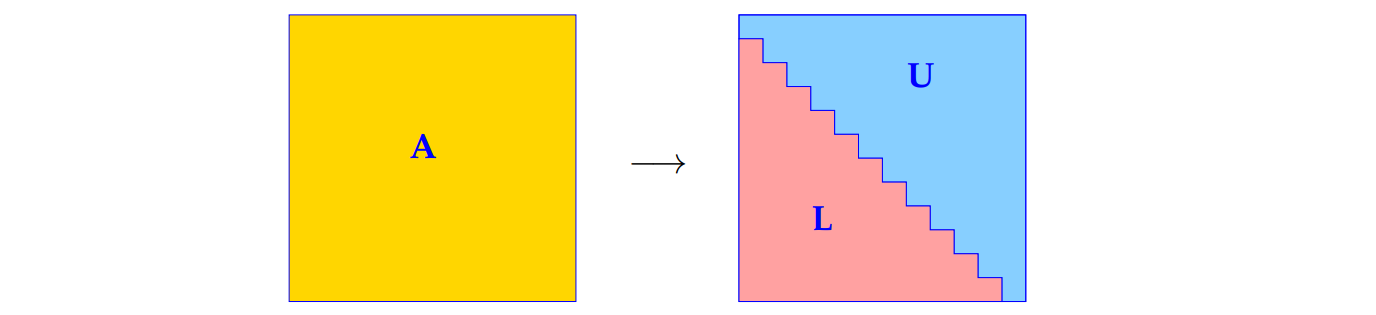
\includegraphics[width=1.0\linewidth]{LUStorage.png}
\end{figure}
We can extract the matrices $\mathbf{L}$ and $\mathbf{U}$ using \verb|matrixLU()| and then calling 
\\[2mm]
\verb|triangularView<Eigen::Upper>()| 
\\[1mm]
or  \\[2mm]
\verb|triangularView<Eigen::StrictlyLower>| \\[1mm]


\paragraph{QR-decomposition:} The QR-decomposition exists for any matrix $\mathbf{A}\in \mathbb{K}^{n,k}$ with $\text{rank}\left(\mathbf{A}\right) = k$. We distinguish two types

\begin{figure}[!hbt]
    \centering
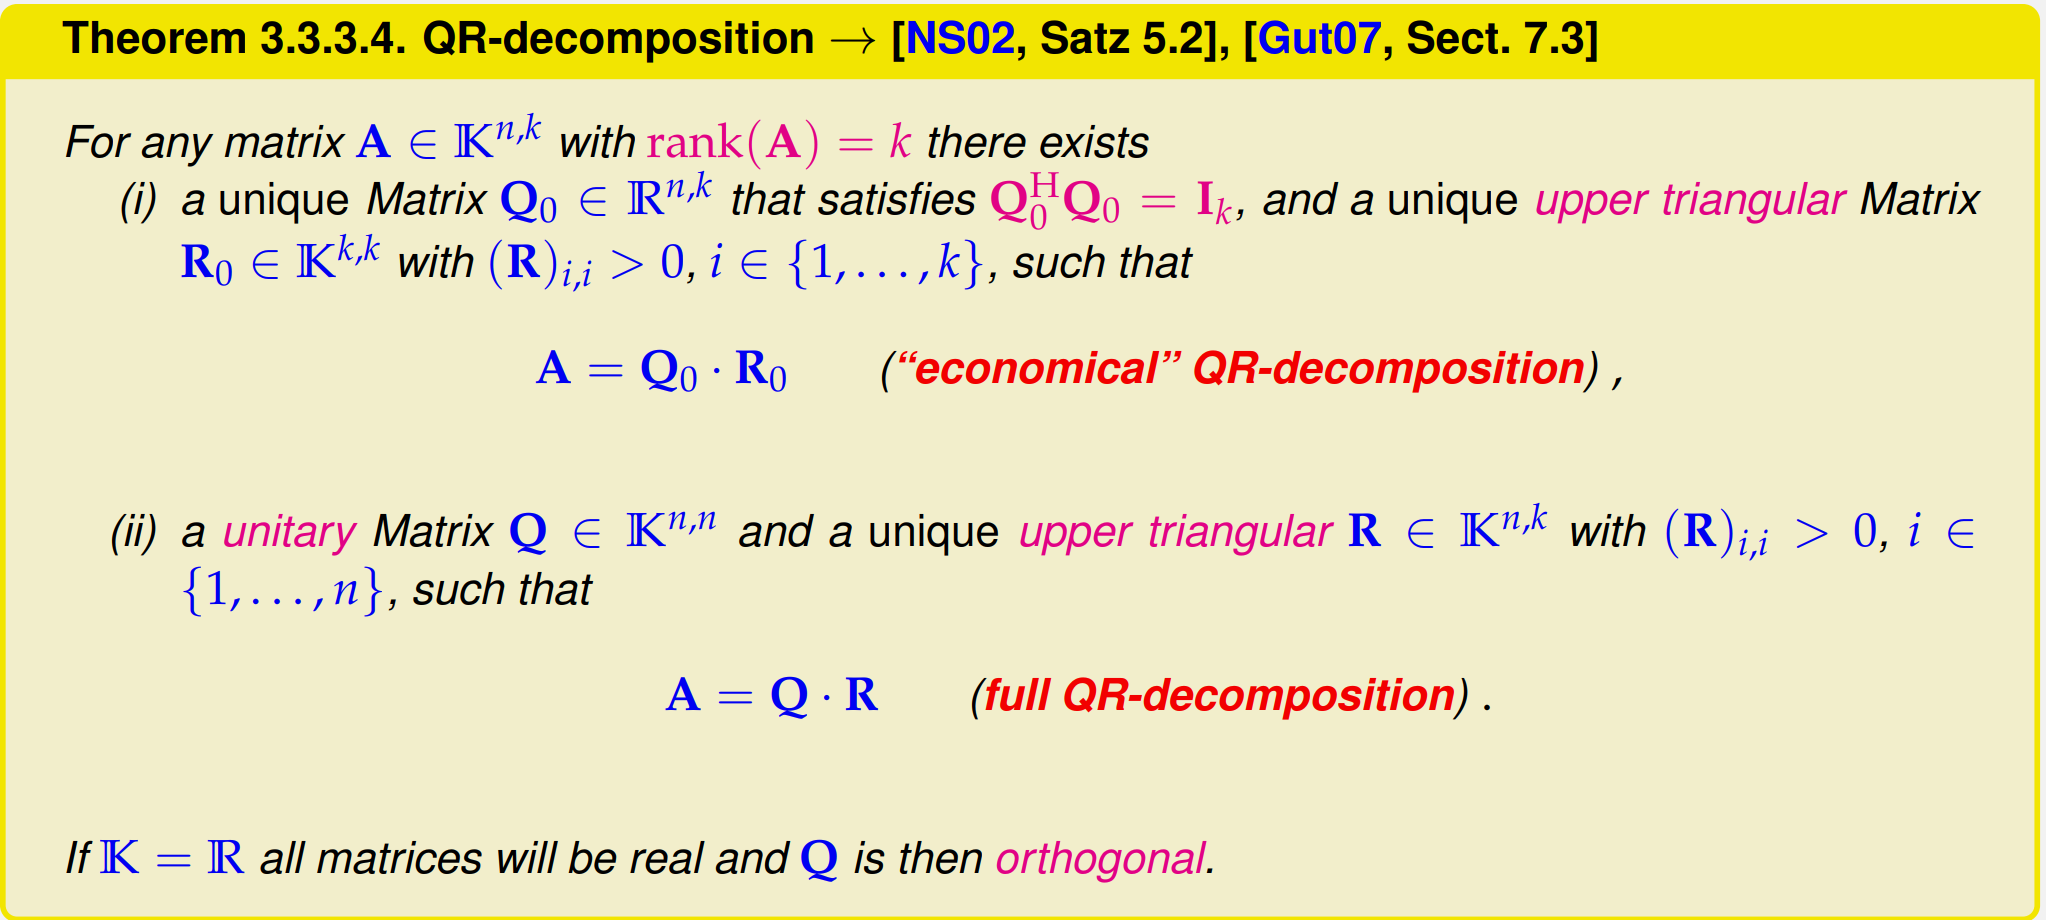
\includegraphics[width=0.8\linewidth]{QR-Decomposition.png}
\end{figure}

\pagebreak

\noindent In Eigen we use the functionality given to us by Householder transformations via \verb|householderQR|, \verb|colPivHouseholderQR| or \verb|fullPivHouseholderQR| to get the QR-decomposition. This will store the matrix $\mathbf{R}$ and the Householder transformations which we can extract using \verb|householderQ()|. The Householder transformations and the matrix $\mathbf{R}$ are both stored in the same matrix. In the case of $m < n$ this looks like

\begin{figure}[!hbt]
    \centering
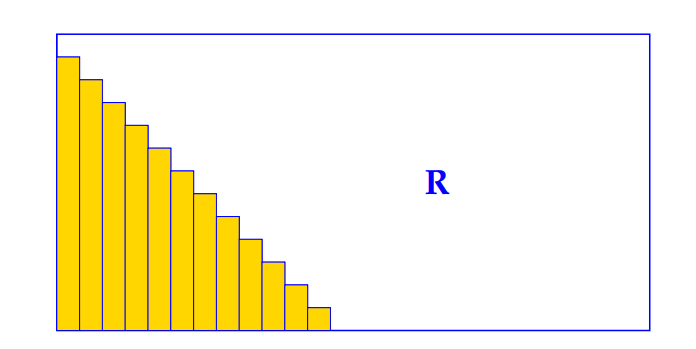
\includegraphics[width=0.4\linewidth]{QRStorage2.png}
\end{figure}

\noindent in the case that $m > n$ this looks like 

\begin{figure}[!hbt]
    \centering
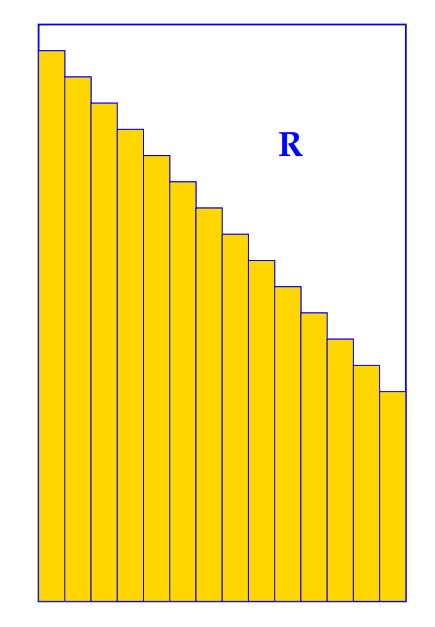
\includegraphics[width=0.2\linewidth]{QRStorage1.png}
\end{figure}

\noindent We can extract the matrix $\mathbf{R}$ using \verb|matrixQR()| which gives us exactly this matrix and then using \verb|triangularView<Eigen::Upper>|. The \verb|householderQR| decomposition for a matrix $\mathbf{A} \in \mathbb{R}^{m,n}$ with $m > n$ is $\mathcal{O}\left(mn^{2}\right)$.

\paragraph{Cholesky decomposition:} For \textbf{symmetric positive definite} matrices  $\mathbf{A}\in \mathbb{K}^{n,n}$ there is a unique upper triangular $\mathbf{R}\in \mathbb{K}^{n,n}$ with $r_{ii} > 0$, $i = 1, \dots, n$, such that $\mathbf{A} = \mathbf{R}^{\mathsf{H}}\mathbf{R}$. We can get this decomposition using \verb|llt()| in Eigen. A decomposition $\mathbf{A} = \mathbf{L}\mathbf{D}\mathbf{L}^{\mathsf{T}}$ where $\mathbf{D}$ is a diagonal matrix with the diagonal entries being the diagonal of $\mathbf{U}$, which follows directly from the LU decomposition of $\mathbf{A}$ is given to us using \verb|ldlt()| and we could get the Cholesky decomposition by setting $\mathbf{R} = \sqrt{\mathbf{D}}\mathbf{L}^{\mathsf{T}}$ seeing as $\mathbf{D}$ has positive diagonal entries. 

\paragraph{SVD:} For any matrix there are unitary / orthogonal matrices $\mathbf{U}\in \mathbb{K}^{m,m}$, $\mathbf{V}\in \mathbb{K}^{n,n}$ and a (generalized, means that it must not necessarily be square) diagonal matrix $\mathbf{\Sigma} = \text{diag}\left(\sigma_{1},\dots, \sigma_{p}\right) \in \mathbb{R}^{m,n}$ and $p:=\text{min}\left\{m,n\right\}$ and $\sigma_{1} \leq \sigma_{2} \leq \dots, \sigma_{p} \leq 0$ such that $\mathbf{A} = \mathbf{U}\mathbf{\Sigma}\mathbf{V}^{\mathsf{H}}$. 

\pagebreak

\noindent We can take the economical singular value decomposition using

\begin{figure}[!hbt]
    \centering
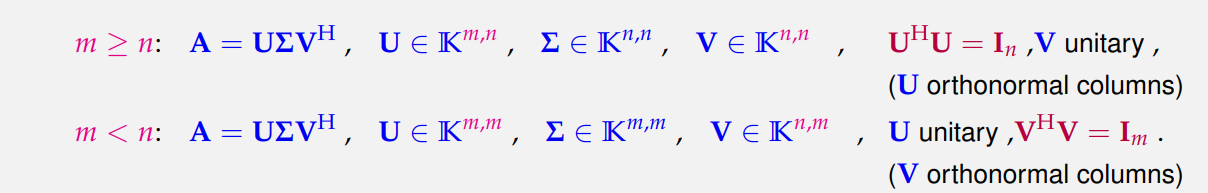
\includegraphics[width=1.0\linewidth]{SVDFatThin.png}
\end{figure}

\noindent In Eigen we can use \\[2mm]
\verb|Eigen::JacobiSVD<Eigen::MatrixXd>| \\[1mm]
to get the singular value decomposition of a matrix. We can use the types \verb|Eigen::ComputeFullU|, \verb|Eigen::ComputeFullV|, \verb|Eigen::ComputeThinU| and  \\ \verb|Eigen::ComputeThinV| in combination with the constructor to get exactly the type of SVD we desire. We can mix these types. For example we could have \\[2mm]
\begin{verbatim}
Eigen::JacobiSVD<Eigen::MatrixXd> SVD(A, Eigen::ComputeThinU | Eigen::ComputeFullV)
\end{verbatim}
We can extract the matrix $\mathbf{U}$ using \verb|matrixU()|, the matrix $\mathbf{V}$ using \verb|matrixV()| and the matrix $\mathbf{\Sigma}$ using \verb|singularValues()|. For a matrix $\mathbf{A}\in \mathbb{K}^{m,n}$ we have the computational cost for the economical SVD as $\mathcal{O}\left(\text{min}\left\{m,n\right\}^{2}\text{max}\left\{m,n\right\}\right)$

\paragraph{$\mathbf{A}$ has special structure:} Sometimes the coefficient matrix $\mathbf{A}$ has a special structure that allows to solve the LSE directly from the given matrix $\mathbf{A}$.

\begin{figure}[!hbt]
    \centering
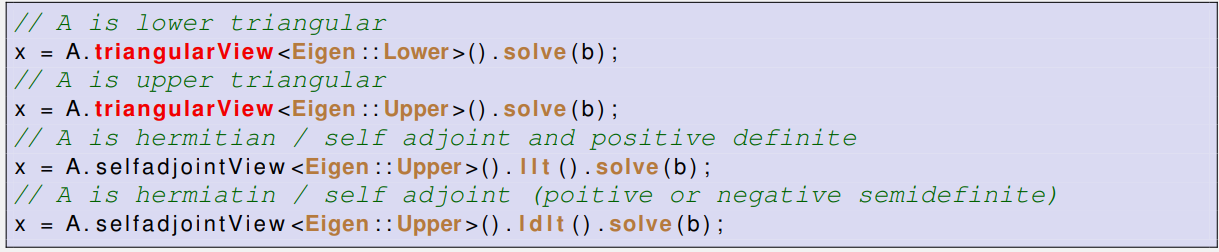
\includegraphics[width=1.0\linewidth]{SpecialStructureMatrices.png}
\end{figure}
An upper / lower triangular system can always be directly solved using \verb|triangularView| which one should keep in mind. 

\pagebreak

\subsection*{2-1.b}
We are now tasked with implementing a method \verb|fruitPrice| which determines from the above information the prices of the fruits in the following order:
\begin{center}
    Mango - Kiwi - Lychee - Banana - Pomegranate - Pineapple
\end{center}
First let us retrieve the coefficient matrix $\mathbf{A}$ and the right side vector $\mathbf{b}$ from the given information.
\begin{equation*}
\mathbf{A} = 
    \begin{bmatrix}
        3 & 1 & 7 & 2 & 0 & 0 \\
        2 & 0 & 0 & 0 & 0 & 1 \\
        1 & 0 & 0 & 0 & 3 & 0 \\
        0 & 5 & 0 & 1 & 0 & 0 \\
        0 & 0 & 0 & 2 & 0 & 1 \\
        0 & 1 & 20 & 0 & 0 & 0
    \end{bmatrix} \quad \mathbf{b} = \begin{bmatrix}
        11.10 \\
        17.00 \\
        \phantom{0}6.10 \\
         \phantom{0}5.25 \\
        12.50 \\
         \phantom{0}7.00
    \end{bmatrix}
\end{equation*}
We then use one of the solvers described above to compute the result, which produces the following code.
\begin{figure}[!hbt]
    \centering
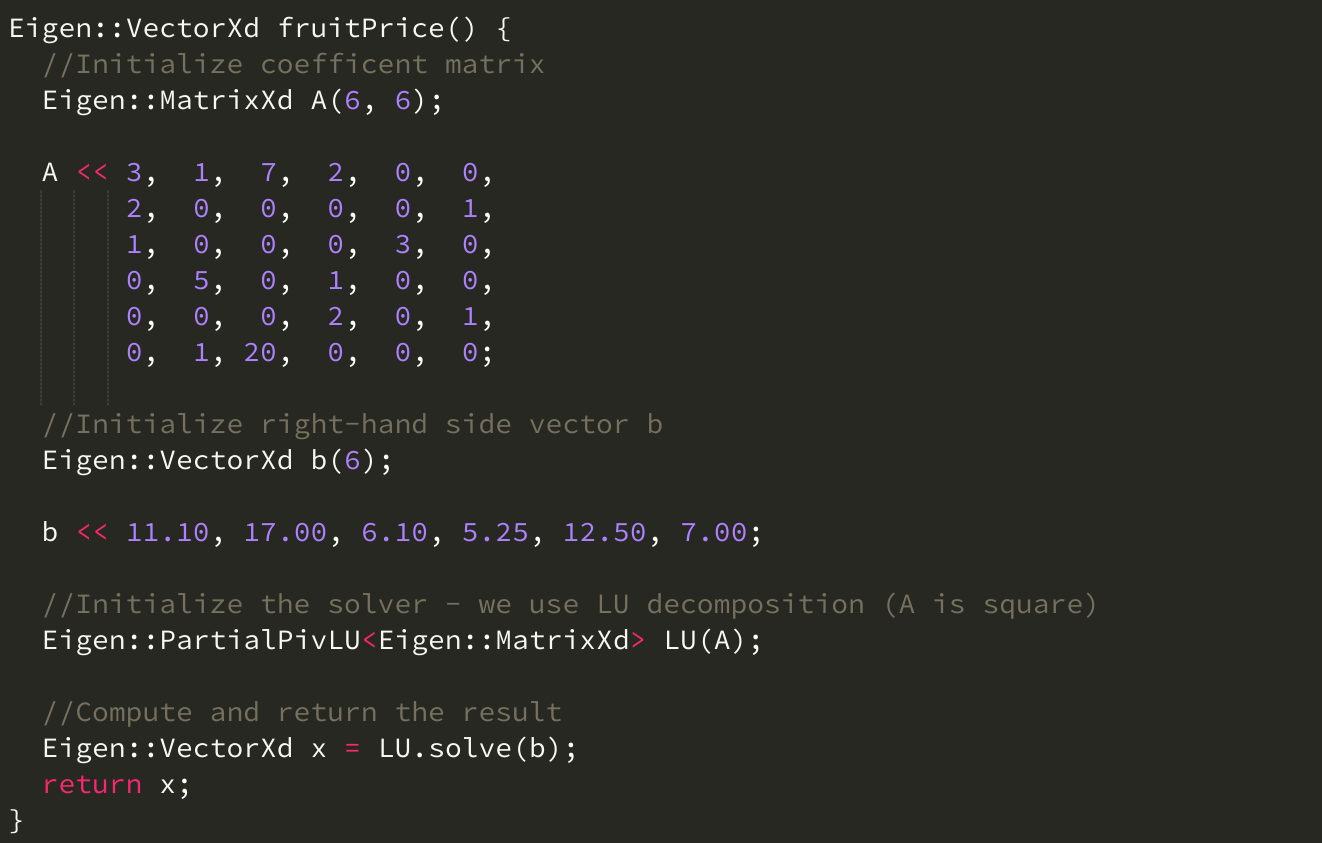
\includegraphics[width=1.0\linewidth]{2-1.b.png}
\end{figure}


\end{document}
